\chapter{Evaluation}
\label{ch:evaluation}
The implementation of the prototype was described in Chapter~\ref{ch:impl}.
This chapter is concerned with testing the procedural version of the WebGL application vs. a non-procedural version, where static assets were used.

To accurately determine the performance of both versions, the codebases were diverged.
When we speak of performance we are considering initialisation time only, as when running the scenes are identical and will perform identically.
This is necessary as for the static assets version, the assets are included in the javascript sent to the client.
Including these in the procedurally generated version would cause unnecessary slowdown in initialisation.
Also, the procedurally generated version has many shaders which are unnecessary for the static assets version and would affect its initialisation time.
We present an explanation of how the performance tests were setup, present the results of the performance test.

We will then compare the output of the program to comparable WebGL games to assess the aesthetic complexity of the scenes created.

\section{Local Performance Test Setup - Static Assets}
The static assets version of the codebase was setup to read in 6 different textures, one for each of the objects in the scene.
Each texture is 1024x1024 in resolution, which is a pretty standard texture size for games theses days.
Popular texture sites such as Mayang's textures have textures with resolution 1600x1200 ~\cite{web:mayangtex}, so I think 1024x1024 is very reasonable.
Since the objects in the scene vary greatly in size it would be possible to texture some objects such as pillars with smaller textures, however this was not done.
All objects use the same shaders to render them, namely the fragment shader in Listing~\ref{lst:withtexfrag} and the vertex shader in Listing~\ref{lst:withtexvert}.
I originally wanted to create a separate bump mapping shader, where the normal information was retrieved from a texture image, however time prevented this.

Once the textures are loaded, the models are retrieved from the assets generated from the design program.
This is described in Section~\ref{sec:staticassetimpl}, and basically involves reading line by line the models and creating WebGL buffers from these, with which we can draw the information.

In our initialisation tests, we also include one call to the ``ModelDrawer.draw()'' function for each, as this will compile and link the shaders.
This is important to consider as compiling and linking shaders takes time, and longer shaders will take longer to compile.
Therefore, for a fair comparison of both procedural and the non-procedural versions, we must make an initial draw call.

\section{Local Performance Test Setup - Procedural Content Generation}
The procedurally generated content version of the codebase does not read in any textures of models, but generates them entirely from scratch.
The process is described in detail in Section~\ref{sec:procgen}, but we will describe here the performance impact of the code executed.

Firstly, what is done is the geometry generation phase is called.
This includes plan generation, plan extrusion, object generation and vertex generation.
There is very little overhead here, all that is required is to set up a few objects and the model information can be generated.
However, once the objects are created, the generation of models is very fast, as there is no expensive string parsing as with the static asset version.
This means that this version will be able to generate content in a more scalable fashion than the static asset version.

The shaders used are far more complex than the ones used for the texture generation process, so the compilation of shaders will take longer.
However this is a linear delay, and should not be affected by the size of the scene generated.

\section{Local Performance Test Results}
This test involved deploying the code locally on a machine with the following specifications:

\begin{itemize}
	\item Gwt version: Gwt 2.3.0
	\item GwtGL version: GwtGL 0.9-SNAPSHOT
	\item Web Browser: Chromium 15.0.849.0 (Developer Build 0 Linux)
	\item Web Server: Apache Tomcat/5.5.33
	\item OS: Linux 3.0-ARCH x86\_64
	\item GPU: Palit Nvidia GeForce GTS 250 1024MB GDDR3 PCI-Express Graphics Card
	\item CPU: Intel Core i7 920 D0 Stepping (SLBEJ) 2.66Ghz (Nehalem)
	\item Mem: Corsair XMS3 4GB (2x2GB) DDR3 PC3-10666C9 1333MHz Triple Channel
	\item HDD: Seagate Barracuda 7200.12 500GB SATA-II 16MB Cache
\end{itemize}

We setup 5 test scenes, with increasingly large numbers of polygons in the scenes.
Each time the number of polygons is doubled.
We tested the initialisation time of the 5 scenes, with initialisation being:
\begin{itemize}
	\item Load each model (From assets or procedurally generating)
	\item Loading Textures (Only for static asset version)
	\item One draw command for each model
\end{itemize}

As we can see from the results in Figure~\ref{fig:perfresultslocal} , the time taken for the initialisation of the static asset scene increases exponentially as the size of the polygons increases.
We can also see that the initialisation time for the procedurally generated scene remains very low regardless of the input size.
We can see that it grows linearly at a very slow pace in comparison to the initialisation of the static assets.

However, for very small scenes of less than 6000 polygons, the static asset version is faster.
This is due to the fact that the procedural version has more overhead when it comes to compiling and linking shaders.
For small scenes, reading in files in a brute force fashion as is done in the static asset version is actually advantageous.

We can therefore conclude that for scenes where the complexity is greater than 6000 polygons, generating content procedurally reduces initialisation time significantly.

\begin{figure}
  \centering
  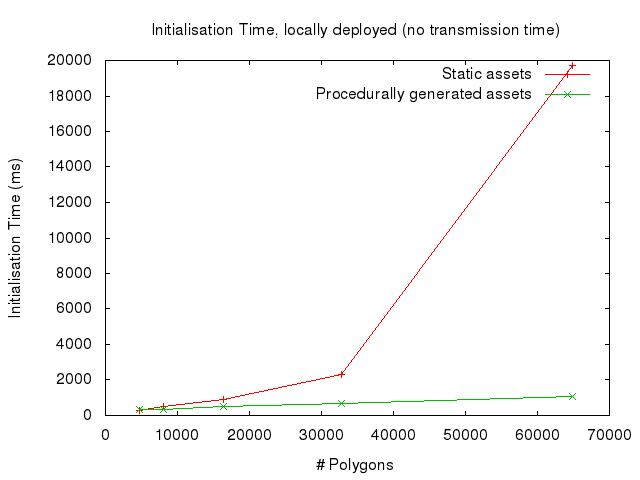
\includegraphics[width=1.0\textwidth]{images/perfresultslocal}
  \caption{Initialisation times for scenes of increasing complexity for both procedurally generated and static asset scenes}
  \label{fig:perfresultslocal}
\end{figure}

%\section{Networked Tests Performance Test Results}
%TODO:
%	>> Different connections
%	>> Different Loading times

\section{Aesthetic Complexity}
When we compare the aesthetics of this prototype, it is important to consider that I am not an artist.
This project has merely shown that procedural effects are possible using the architecture that is presented.
It is hoped that artists will build upon the work presented here to create vastly greater effects.

That said, it compares reasonably against current generation WebGL such as is seen in Figure~\ref{fig:minevstank} where a screenshot from this demo is compared against a screenshot from TankWorld, a current WebGL Game~\cite{web:tankworld}.
As can be seen, the tankworld game contains fairly bland colours and textures, whereas my prototype contains more colourful textures, especially the skybox.
However, my demo does not have any lighting effects like shadowns that TankWorld has, but it does have bump mapping which TankWorld does not have.

It should be said that although this prototype does not present graphically everything that procedural generation can offer, it does compare reasonably against modern WebGL games.

\begin{figure}
  \centering
  \subcaptionbox{My Solution}{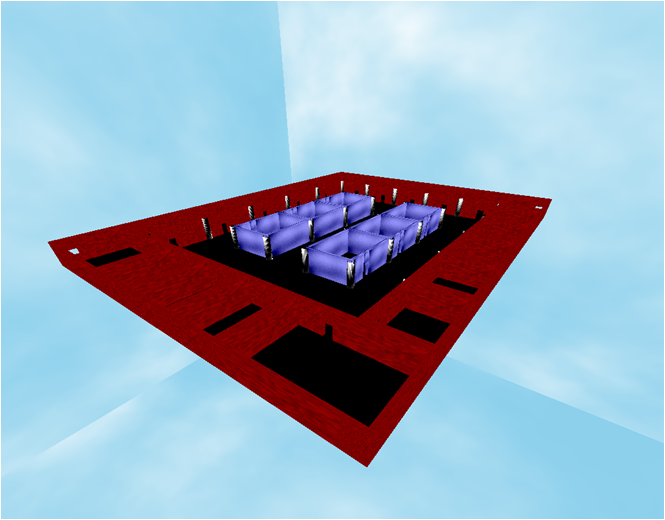
\includegraphics[width=0.5\textwidth]{images/procgl}}
  \subcaptionbox{TankWorld WebGL Game}{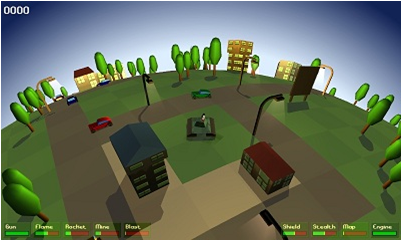
\includegraphics[width=0.5\textwidth]{images/tankworld}}
  \caption{Comparison screenshots from my prototype and a screenshot from TankWorld, a current WebGL game.}
  \label{fig:minevstank}
\end{figure}

\section{Design Program Simplicity}
\label{sec:designsimplicity}
As shown in Figure~\ref{fig:designapp}, a wide variety of scenes can be generated by changing a small number of parameters.
However to add new models it is required to create a subclass of the Entity subclass and implement the necessary functions.
This should be relatively straightforward for anyone with a knowledge of Java or Object Oriented programming, as Processing is a simple framework to use.

To create compound models, the user does not need to create new classes however, they can use the existing primitives which exist.
An interactive Gui would help with this, but there is no reason why objects like chairs, desks, shelves, etc. cannot be implemented as a combination of cuboids and cylinders.
Indeed this is an area of future work for this project.

\section{Extensibility}
Project extensibility is a big factor in everything that was accomplished in this project.
This is the first framework for procedural content generation for WebGL that the author is aware of.
It is also highly generic and it could easily be ported to desktop OpenGL or OpenGL ES 2.0 on mobile with little effort.

Nearly every part of the codebase is highly extensible.
Indeed writing new shaders is very simple, we simply need to write them and include them in the maven project and reference them in the model we want to use them for.
As said in Section~\ref{sec:designsimplicity} to extend models we simply subclass the Entity and come up with some way of generating the quads that are needed.
The entity class already has a lot of useful functions for generating models such as cuboids, so it would be trivial to create new models using these methods.

\section{Research Contribution}
I believe what is offered here is more than just an implementation of just procedural techniques in WebGL.
We have presented a generic framework for generating procedural content in WebGL.
The incorporation of both geometric and texture generation into a unified pipeline is unique in this project.

The sample programs created and tested are proof of the utility of this framework.
It also acts as a proof of concept that procedural content generation can be of benefit to anyone implementing games on this new platform, especially the vastly decreased loading times which players will experience with procedurally generated content over loading static assets.
